\begin{center}

\includegraphics[width=0.5\textwidth]{content/3/chapter4/images/47.png}\\
Cippi在上楼梯
\end{center}

本节介绍C++20核心语言中其余的改进。

\subsubsubsection{4.9.1\hspace{0.2cm}volatile}

\href{http://www.open-std.org/jtc1/sc22/wg21/docs/papers/2018/p1152r0.html}{P1152R0}提案摘要概述了volatile所经历的变化:“建议弃用volatile的部分用法,并删除不明确的部分的用法”\href{https://www.zhihu.com/question/366070396}{知乎上的讨论}。这篇文章的目的在于,在运行时或编译器更新时已经出现了微妙损坏的代码,使用volatile的不明确行为时,会使编译时代码遭到破坏。”深入讨论volatile之前,我想回答一个关键问题:什么时候应该使用volatile?

C++标准的某个注释:“volatile是对实现的一个提示,以避免进行激进地优化,因为对象的值可会通过实现无法检测到的方式改变。”所以对于单线程,编译器必须在可执行文件中执行加载或存储操作,就像源码中一样频繁,所以volatile不能消除或重新排序。因此,可以使用volatile对象与处理程序通信,但不能用于与另一个执行线程通信。

展示volatile保留了哪些语义之前,我想先从已弃用的特性开始说起:

\begin{enumerate}
\item 
弃用volatile的复合赋值,以及前后递增/递减

\item 
弃用函数参数或返回类型的volatile限定

\item 
结构化绑定声明中弃用volatile限定符
\end{enumerate}

若想知道背后复杂的细节,我建议你观看一下CppCon 2019的演讲\href{https://www.youtube.com/watch?v=KJW_DLaVXIY}{“废除volatile”}。下面是他演讲中的几个例子,我修复了源码中的一些拼写错误。下面代码片段中的数字代表前面列出的三个弃用语义。

\hspace*{\fill} \\ %插入空行
\noindent
\textbf{弃用的volatile用例}
\begin{lstlisting}[style=styleCXX]
// (1)
int neck, tail;
volatile int brachiosaur;
brachiosaur = neck; // OK, a volatile store
tail = brachiosaur; // OK, a volatile load

// deprecated: does this access brachiosaur once or twice
tail = brachiosaur = neck;

// deprecated: does this access brachiosaur once or twice
brachiosaur += neck;

// OK, a volatile load, an addition, a volatile store
brachiosaur = brachiosaur + neck;

#########################################
// (2)
// deprecated: a volatile return type has no meaning
volatile struct amber jurassic();

// deprecated: volatile parameters aren't meaningful to the
// caller, volatile only applies within the function
void trex(volatile short left_arm, volatile short right_arm);

// OK, the pointer isn't volatile, the data it points to is
void fly(volatile struct pterosaur* pterandon);

########################################
(3)
struct linhenykus { volatile short forelimb; };
void park(linhenykus alvarezsauroid) {
	// deprecated: does the binding copy the forelimbs?
	auto [what_is_this] = alvarezsauroid; // structured binding
	// ...
}
\end{lstlisting}

\begin{tcolorbox}[breakable,enhanced jigsaw,colback=red!5!white,colframe=red!75!black,title={volatile和多线程语义}]
volatile通常用于表示,独立于常规程序流,并可以进行修改的对象。例如,这些是嵌入式编程中表示外部设备(内存映射I/O)的对象。因为这些对象可以独立于常规程序流进行修改,并且它值直接写入主存,因此缓存中不会进行优化存储。简单来说,volatile避免了主动优化,并且没有多线程语义。
\end{tcolorbox}

\subsubsubsection{4.9.2\hspace{0.2cm}带有初始化式的范围for循环}

C++20可以直接使用带有初始化式的范围for循环。

\begin{lstlisting}[style=styleCXX]
// rangeBasedForLoopInitializer.cpp

#include <iostream>
#include <string>
#include <vector>

int main() {

	for (auto vec = std::vector{1, 2, 3}; auto v : vec) {
		std::cout << v << " ";
	}
	
	std::cout << "\n\n";
	
	for (auto initList = {1, 2, 3}; auto e : initList) {
		e *= e;
		std::cout << e << " ";
	}
	
	std::cout << "\n\n";
	
	using namespace std::string_literals;
	for (auto str = "Hello World"s; auto c: str) {
		std::cout << c << " ";
	}
	
	std::cout << '\n';

}
\end{lstlisting}

基于范围的for循环在第9行使用std::vector,第15行使用std::initializer\_list,第23行使用std::string。此外,第9行和第15行中,类模板使用了C++17的自动类型推断(使用std::vector,而非std::vector<int>)。

\begin{tcblisting}{commandshell={}}
1 2 3

1 4 9

H e l l o  W o r l d
\end{tcblisting}

\subsubsubsection{4.9.3\hspace{0.2cm}virtual constexpr函数}

constexpr函数有可能在编译时执行,但也可以在运行时执行。因此,可以使用C++20的virtual关键字创建constexpr函数。virtual的constexpr函数可以重写为非constexpr函数,virtual的非constexpr函数可以重写virtual的constexpr函数。在这里,重写意味着基类的相关函数是虚函数。

virtualconstexr.cpp展示了这两种组合:

\begin{lstlisting}[style=styleCXX]
// virtualConstexpr.cpp

#include <iostream>

struct X1 {
	virtual int f() const = 0;
};

struct X2: public X1 {
	constexpr int f() const override { return 2; }
};

struct X3: public X2 {
	int f() const override { return 3; }
};

struct X4: public X3 {
	constexpr int f() const override { return 4; }
};

int main() {
	
	X1* x1 = new X4;
	std::cout << "x1->f(): " << x1->f() << '\n';
	
	X4 x4;
	X1& x2 = x4;
	std::cout << "x2.f(): " << x2.f() << '\n';

}
\end{lstlisting}

第24行通过指针使用虚函数(后期绑定),第28行通过引用使用虚函数。

\begin{tcblisting}{commandshell={}}
x1->f(): 4
x2.f(): 4
\end{tcblisting}

\subsubsubsection{4.9.4\hspace{0.2cm}UTF-8字符串的新字符类型:char8\_t}

除了C++11中的字符类型char16\_t和char32\_t外,C++20添加了新的字符类型char8\_t。类型char8\_t足够大,可以表示任何UTF-8单位(8位)。其具有与unsigned char相同的大小、符号和对齐方式,但这是两个不同的类型。

\begin{tcolorbox}[breakable,enhanced jigsaw,colback=blue!5!white,colframe=blue!75!black,title={char和char8\_t}]

与char8\_t相反,char有一个字节,一个字节的比特数,并且char的比特数没有明确定义。不过,几乎所有的实现都使用8位作为一个字节。char类型的std::basic\_string,别名为std::string。

\hspace*{\fill} \\ %插入空行
\noindent
\textbf{std::string和std::string字面值}
\begin{lstlisting}[style=styleCXX]
std::string std::basic_string<char>
"Hello World"s
\end{lstlisting}
\end{tcolorbox}

因此,C++20有一个新的字符类型char8\_t(第1行)和新的UTF-8字符串字面值(第2行)。

\hspace*{\fill} \\ %插入空行
\noindent
\textbf{新的char8\_t字符类型和UTF-8字面值}
\begin{lstlisting}[style=styleCXX]
std::u8string std::basic_string<char8_t>
u8"Hello World"
\end{lstlisting}

char8Str.cpp展示了新字符类型char8\_t的用法。

\begin{lstlisting}[style=styleCXX]
// char8Str.cpp

#include <iostream>
#include <string>

int main() {
	
	const char8_t* char8Str = u8"Hello world";
	std::basic_string<char8_t> char8String = u8"helloWorld";
	std::u8string char8String2 = u8"helloWorld";
	
	char8String2 += u8".";
	
	std::cout << "char8String.size(): " << char8String.size() << '\n';
	std::cout << "char8String2.size(): " << char8String2.size() << '\n';
	
	char8String2.replace(0, 5, u8"Hello ");
	
	std::cout << "char8String2.size(): " << char8String2.size() << '\n';

}
\end{lstlisting}

下面是程序的输出:

\begin{tcblisting}{commandshell={}}
char8String.size(): 10
char8String2.size(): 11
char8String2.size(): 12
\end{tcblisting}

\subsubsubsection{4.9.5\hspace{0.2cm}本地作用域中的using enum}

using enum声明在局部作用域中引入已命名枚举的枚举值。

\hspace*{\fill} \\ %插入空行
\noindent
\textbf{本地作用域内引入枚举值}
\begin{lstlisting}[style=styleCXX]
// enumUsing.cpp

#include <iostream>
#include <string_view>

enum class Color {
	 red,
	 green,
	 blue
};

std::string_view toString(Color col) {
	switch (col) {
		using enum Color;
		case red: return "red";
		case green: return "green";
		case blue: return "blue";
	}
	return "unknown";
}

int main() {

	std::cout << '\n';
	
	std::cout << "toString(Color::red): " << toString(Color::red) << '\n';
	
	using enum Color;
	
	std::cout << "toString(green): " << toString(green) << '\n';
	
	std::cout << '\n';

}
\end{lstlisting}

using enum声明(第14行)将作用域enumeration Color的枚举值引入到本地作用域,从而枚举值可以无作用域的进行使用(第15-17行)。

\begin{center}
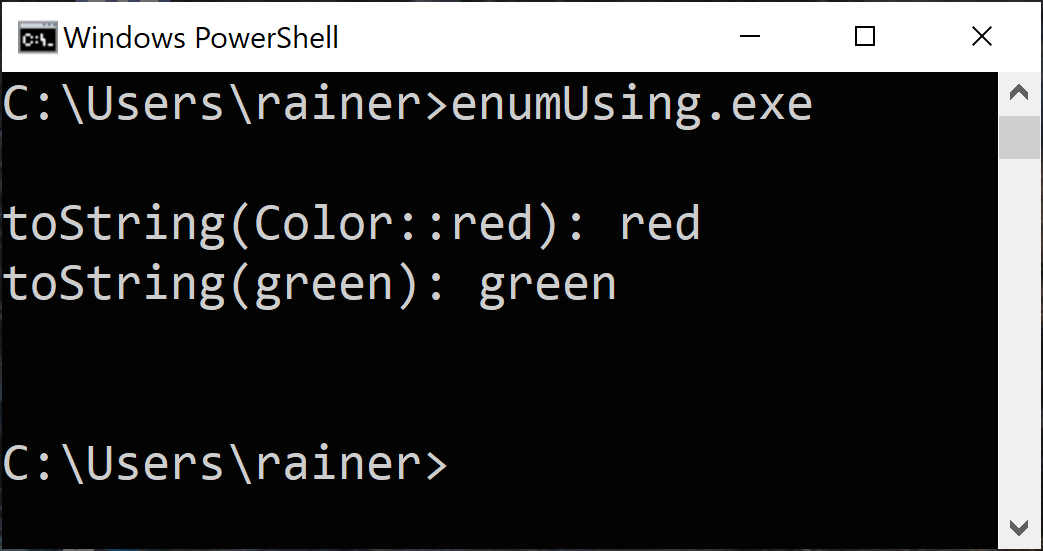
\includegraphics[width=0.4\textwidth]{content/3/chapter4/images/48.png}\\
使用using enum
\end{center}

\subsubsubsection{4.9.6\hspace{0.2cm}位域成员变量的默认初始化器}

首先,什么是位域?下面是来自\href{https://en.wikipedia.org/wiki/Bit_field}{Wikipedia}: “位域是计算机编程中的数据结构,由许多相邻的计算机内存位置组成,这些位置可用来保存一组位值,存储的目的是使该集合中的单个位或一组位都可以寻址。位域常用来表示固定宽度的整型。”

C++20可以默认初始化位域成员变量:

\begin{lstlisting}[style=styleCXX]
// bitField.cpp

#include <iostream>

struct Class11 {
	int i = 1;
	int j = 2;
	int k = 3;
	int l = 4;
	int m = 5;
	int n = 6;
};

struct BitField20 {
	int i : 3 = 1;
	int j : 4 = 2;
	int k : 5 = 3;
	int l : 6 = 4;
	int m : 7 = 5;
	int n : 7 = 6;
};

int main () {
	
	std::cout << '\n';
	
	std::cout << "sizeof(Class11): " << sizeof(Class11) << '\n';
	std::cout << "sizeof(BitField20): " << sizeof(BitField20) << '\n';
	
	std::cout << '\n';

}
\end{lstlisting}

C++11中,根据类的成员(第6-11行),位域成员可以有默认的初始化器(第15-20行)。当把3、4、5、6、7、7这些数字加起来时,会得到32。因此,32位或4字节恰好是BitField20的大小:

\begin{center}
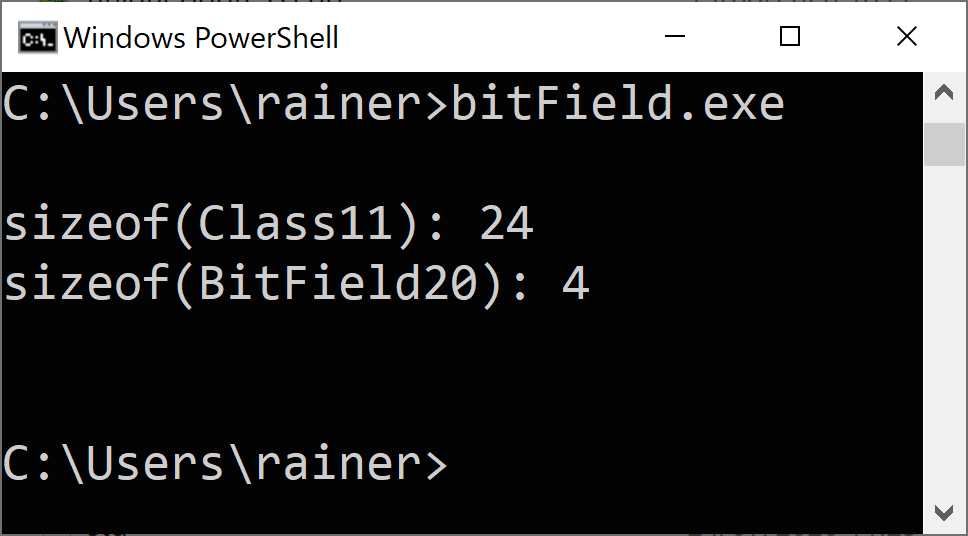
\includegraphics[width=0.4\textwidth]{content/3/chapter4/images/49.png}\\
位域的大小
\end{center}

\begin{tcolorbox}[breakable,enhanced jigsaw,colback=mygreen!5!white,colframe=mygreen!75!black,title={总结}]
\begin{itemize}
\item 
C++20中明确了volatile的行为。volatile没有多线程语义,应仅用于避免激进优化,因为对象可能独立于常规程序流,并且可以进行修改。

\item 
基于范围的for循环可以使用初始化式。

\item 
新的字符类型char8\_t足够大,明确可以表示8位。

\item 
using enum声明在本地作用域中引入了命名枚举的枚举值。

\item 
位域的成员可以默认初始化。

\item 
constexpr函数可以是虚函数。
\end{itemize}
\end{tcolorbox}























